\documentclass[tikz, border=10pt]{standalone}
\usepackage[utf8]{inputenc}
\usepackage[T1]{fontenc}

\usepackage{fontspec}
\setmainfont{EB Garamond}[
    Ligatures=TeX,
    UprightFont = * Regular,
    ItalicFont = * Italic,
    BoldFont = * SemiBold,
    BoldItalicFont = * SemiBold Italic,
]


\usepackage{xcolor}

\begin{document}

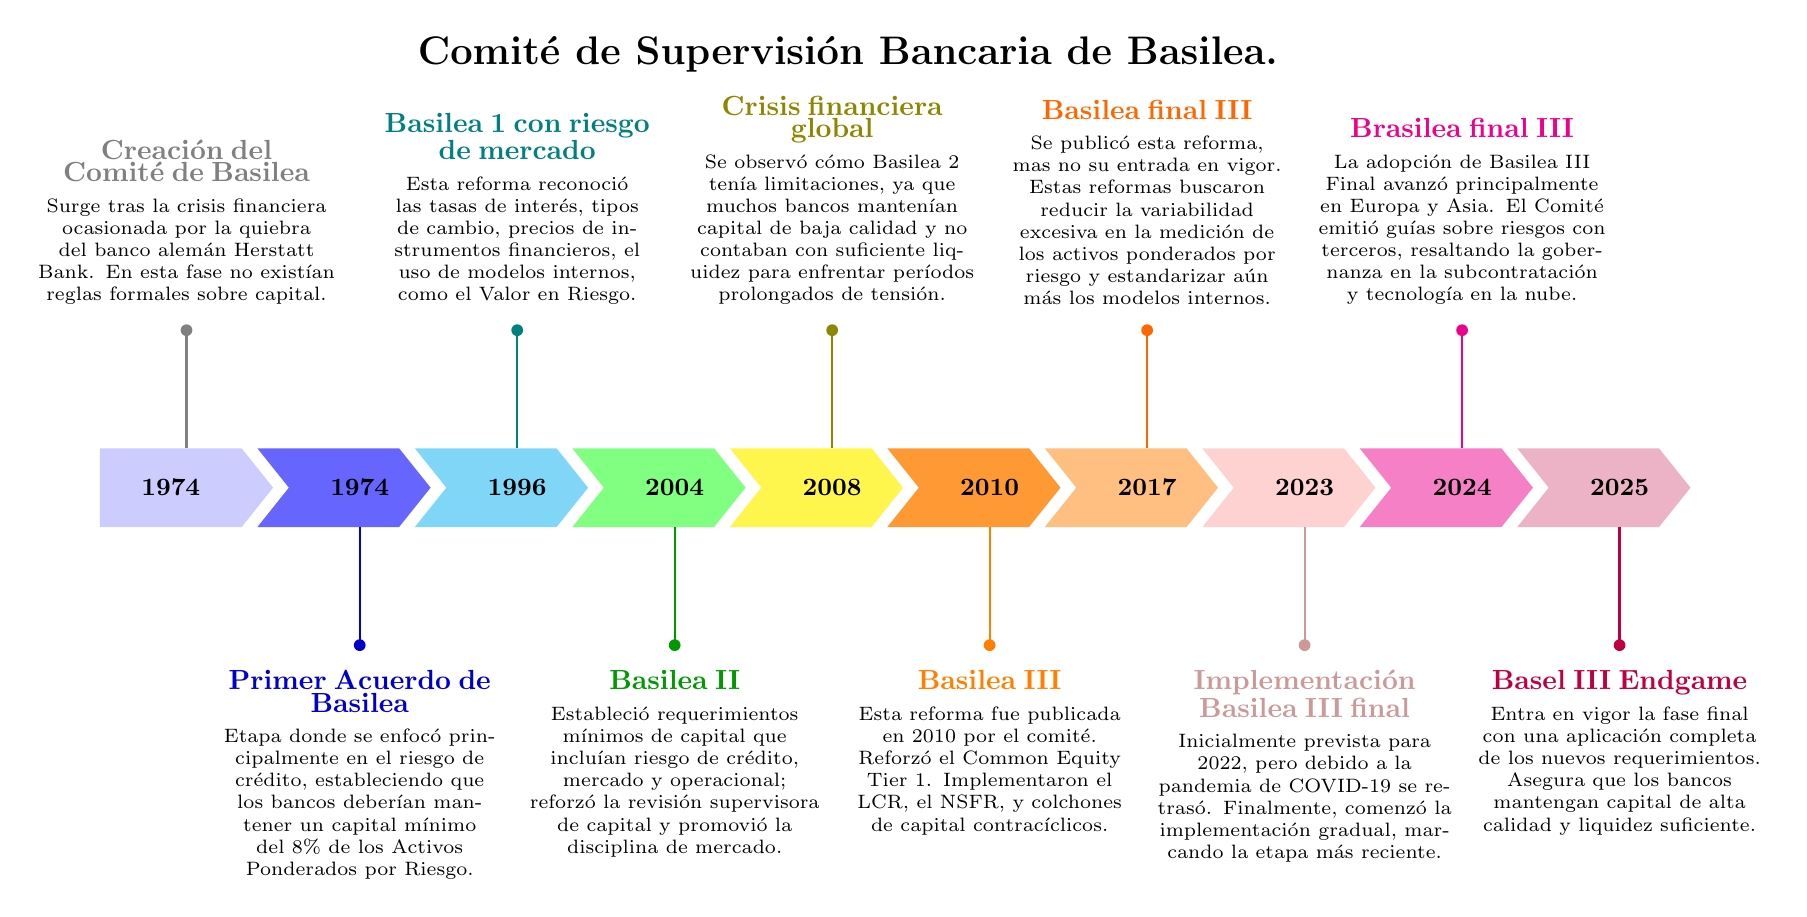
\begin{tikzpicture}[
    event node/.style = {align=center, text width=3.8cm, font=\scriptsize}
]

% Título Principal
\node[font=\Large\bfseries, align=center] at (9.5, 6) {Comité de Supervisión Bancaria de Basilea.};

% --- LÍNEA DE TIEMPO BASE ---
% 1974 - Creación (Inicio plano como en la imagen)
\fill[blue!20] (0,0) -- (1.8,0) -- (2.2,0.5) -- (1.8,1) -- (0,1) -- cycle;
\node[font=\small\bfseries] at (0.9, 0.5) {1974};

% Resto de flechas del timeline
\foreach \x/\year/\clr in {
    2/1974/blue!60, 
    4/1996/cyan!50, 
    6/2004/green!50, 
    8/2008/yellow!70, 
    10/2010/orange!80, 
    12/2017/orange!50, 
    14/2023/pink!70, 
    16/2024/magenta!50, 
    18/2025/purple!30%
} {
    \fill[\clr] (\x,0) -- (\x+1.8,0) -- (\x+2.2,0.5) -- (\x+1.8,1) -- (\x,1) -- (\x+0.4,0.5) -- cycle;
    \node[font=\small\bfseries] at (\x+1.3, 0.5) {\year};
}

% --- FUNCIONES PARA DIBUJAR EVENTOS ---
% Función para eventos superiores: \drawtop{pos_x}{color}{Titulo}{Descripcion}
\def\drawtop#1#2#3#4{
    \draw[#2, thick] (#1, 1) -- (#1, 2.5) node[circle, fill=#2, inner sep=1.5pt] {};
    \node[event node, anchor=south] at (#1, 2.7) {
        \textcolor{#2}{\textbf{\normalsize #3}}\\[1ex]
        #4
    };
}

% Función para eventos inferiores: \drawbot{pos_x}{color}{Titulo}{Descripcion}
\def\drawbot#1#2#3#4{
    \draw[#2, thick] (#1, 0) -- (#1, -1.5) node[circle, fill=#2, inner sep=1.5pt] {};
    \node[event node, anchor=north] at (#1, -1.7) {
        \textcolor{#2}{\textbf{\normalsize #3}}\\[1ex]
        #4
    };
}

% --- LLAMADAS A LOS EVENTOS ---
% --- Superiores ---
\drawtop{1.1}{gray}{Creación del\\ Comité de Basilea}{Surge tras la crisis financiera ocasionada por la quiebra del banco alemán Herstatt Bank. En esta fase no existían reglas formales sobre capital.}

\drawtop{5.3}{teal}{Basilea 1 con riesgo\\ de mercado}{Esta reforma reconoció las tasas de interés, tipos de cambio, precios de instrumentos financieros, el uso de modelos internos, como el Valor en Riesgo.}

\drawtop{9.3}{olive}{Crisis financiera\\ global}{Se observó cómo Basilea 2 tenía limitaciones, ya que muchos bancos mantenían capital de baja calidad y no contaban con suficiente liquidez para enfrentar períodos prolongados de tensión.}

\drawtop{13.3}{orange!80!red}{Basilea final III}{Se publicó esta reforma, mas no su entrada en vigor. Estas reformas buscaron reducir la variabilidad excesiva en la medición de los activos ponderados por riesgo y estandarizar aún más los modelos internos.}

\drawtop{17.3}{magenta}{Brasilea final III}{La adopción de Basilea III Final avanzó principalmente en Europa y Asia. El Comité emitió guías sobre riesgos con terceros, resaltando la gobernanza en la subcontratación y tecnología en la nube.}

% --- Inferiores ---
\drawbot{3.3}{blue!80!black}{Primer Acuerdo de\\ Basilea}{Etapa donde se enfocó principalmente en el riesgo de crédito, estableciendo que los bancos deberían mantener un capital mínimo del 8\% de los Activos Ponderados por Riesgo.}

\drawbot{7.3}{green!60!black}{Basilea II}{Estableció requerimientos mínimos de capital que incluían riesgo de crédito, mercado y operacional; reforzó la revisión supervisora de capital y promovió la disciplina de mercado.}

\drawbot{11.3}{orange}{Basilea III}{Esta reforma fue publicada en 2010 por el comité. Reforzó el Common Equity Tier 1. Implementaron el LCR, el NSFR, y colchones de capital contracíclicos.}

\drawbot{15.3}{pink!80!black}{Implementación\\ Basilea III final}{Inicialmente prevista para 2022, pero debido a la pandemia de COVID-19 se retrasó. Finalmente, comenzó la implementación gradual, marcando la etapa más reciente.}

\drawbot{19.3}{purple}{Basel III Endgame}{Entra en vigor la fase final con una aplicación completa de los nuevos requerimientos. Asegura que los bancos mantengan capital de alta calidad y liquidez suficiente.}

\end{tikzpicture}
\end{document}